
\documentclass{article} % For LaTeX2e
\usepackage{rl_paper,times}
\usepackage{booktabs}
\usepackage{graphicx}
\usepackage{algorithm}
\usepackage{algpseudocode}
\usepackage{float}
\usepackage{enumitem}

% Optional math commands from https://github.com/goodfeli/dlbook_notation.
%%%%% NEW MATH DEFINITIONS %%%%%

\usepackage{amsmath,amsfonts,bm}

% Mark sections of captions for referring to divisions of figures
\newcommand{\figleft}{{\em (Left)}}
\newcommand{\figcenter}{{\em (Center)}}
\newcommand{\figright}{{\em (Right)}}
\newcommand{\figtop}{{\em (Top)}}
\newcommand{\figbottom}{{\em (Bottom)}}
\newcommand{\captiona}{{\em (a)}}
\newcommand{\captionb}{{\em (b)}}
\newcommand{\captionc}{{\em (c)}}
\newcommand{\captiond}{{\em (d)}}

% Highlight a newly defined term
\newcommand{\newterm}[1]{{\bf #1}}


% Figure reference, lower-case.
\def\figref#1{figure~\ref{#1}}
% Figure reference, capital. For start of sentence
\def\Figref#1{Figure~\ref{#1}}
\def\twofigref#1#2{figures \ref{#1} and \ref{#2}}
\def\quadfigref#1#2#3#4{figures \ref{#1}, \ref{#2}, \ref{#3} and \ref{#4}}
% Section reference, lower-case.
\def\secref#1{section~\ref{#1}}
% Section reference, capital.
\def\Secref#1{Section~\ref{#1}}
% Reference to two sections.
\def\twosecrefs#1#2{sections \ref{#1} and \ref{#2}}
% Reference to three sections.
\def\secrefs#1#2#3{sections \ref{#1}, \ref{#2} and \ref{#3}}
% Reference to an equation, lower-case.
\def\eqref#1{equation~\ref{#1}}
% Reference to an equation, upper case
\def\Eqref#1{Equation~\ref{#1}}
% A raw reference to an equation---avoid using if possible
\def\plaineqref#1{\ref{#1}}
% Reference to a chapter, lower-case.
\def\chapref#1{chapter~\ref{#1}}
% Reference to an equation, upper case.
\def\Chapref#1{Chapter~\ref{#1}}
% Reference to a range of chapters
\def\rangechapref#1#2{chapters\ref{#1}--\ref{#2}}
% Reference to an algorithm, lower-case.
\def\algref#1{algorithm~\ref{#1}}
% Reference to an algorithm, upper case.
\def\Algref#1{Algorithm~\ref{#1}}
\def\twoalgref#1#2{algorithms \ref{#1} and \ref{#2}}
\def\Twoalgref#1#2{Algorithms \ref{#1} and \ref{#2}}
% Reference to a part, lower case
\def\partref#1{part~\ref{#1}}
% Reference to a part, upper case
\def\Partref#1{Part~\ref{#1}}
\def\twopartref#1#2{parts \ref{#1} and \ref{#2}}

\def\ceil#1{\lceil #1 \rceil}
\def\floor#1{\lfloor #1 \rfloor}
\def\1{\bm{1}}
\newcommand{\train}{\mathcal{D}}
\newcommand{\valid}{\mathcal{D_{\mathrm{valid}}}}
\newcommand{\test}{\mathcal{D_{\mathrm{test}}}}

\def\eps{{\epsilon}}


% Random variables
\def\reta{{\textnormal{$\eta$}}}
\def\ra{{\textnormal{a}}}
\def\rb{{\textnormal{b}}}
\def\rc{{\textnormal{c}}}
\def\rd{{\textnormal{d}}}
\def\re{{\textnormal{e}}}
\def\rf{{\textnormal{f}}}
\def\rg{{\textnormal{g}}}
\def\rh{{\textnormal{h}}}
\def\ri{{\textnormal{i}}}
\def\rj{{\textnormal{j}}}
\def\rk{{\textnormal{k}}}
\def\rl{{\textnormal{l}}}
% rm is already a command, just don't name any random variables m
\def\rn{{\textnormal{n}}}
\def\ro{{\textnormal{o}}}
\def\rp{{\textnormal{p}}}
\def\rq{{\textnormal{q}}}
\def\rr{{\textnormal{r}}}
\def\rs{{\textnormal{s}}}
\def\rt{{\textnormal{t}}}
\def\ru{{\textnormal{u}}}
\def\rv{{\textnormal{v}}}
\def\rw{{\textnormal{w}}}
\def\rx{{\textnormal{x}}}
\def\ry{{\textnormal{y}}}
\def\rz{{\textnormal{z}}}

% Random vectors
\def\rvepsilon{{\mathbf{\epsilon}}}
\def\rvtheta{{\mathbf{\theta}}}
\def\rva{{\mathbf{a}}}
\def\rvb{{\mathbf{b}}}
\def\rvc{{\mathbf{c}}}
\def\rvd{{\mathbf{d}}}
\def\rve{{\mathbf{e}}}
\def\rvf{{\mathbf{f}}}
\def\rvg{{\mathbf{g}}}
\def\rvh{{\mathbf{h}}}
\def\rvu{{\mathbf{i}}}
\def\rvj{{\mathbf{j}}}
\def\rvk{{\mathbf{k}}}
\def\rvl{{\mathbf{l}}}
\def\rvm{{\mathbf{m}}}
\def\rvn{{\mathbf{n}}}
\def\rvo{{\mathbf{o}}}
\def\rvp{{\mathbf{p}}}
\def\rvq{{\mathbf{q}}}
\def\rvr{{\mathbf{r}}}
\def\rvs{{\mathbf{s}}}
\def\rvt{{\mathbf{t}}}
\def\rvu{{\mathbf{u}}}
\def\rvv{{\mathbf{v}}}
\def\rvw{{\mathbf{w}}}
\def\rvx{{\mathbf{x}}}
\def\rvy{{\mathbf{y}}}
\def\rvz{{\mathbf{z}}}

% Elements of random vectors
\def\erva{{\textnormal{a}}}
\def\ervb{{\textnormal{b}}}
\def\ervc{{\textnormal{c}}}
\def\ervd{{\textnormal{d}}}
\def\erve{{\textnormal{e}}}
\def\ervf{{\textnormal{f}}}
\def\ervg{{\textnormal{g}}}
\def\ervh{{\textnormal{h}}}
\def\ervi{{\textnormal{i}}}
\def\ervj{{\textnormal{j}}}
\def\ervk{{\textnormal{k}}}
\def\ervl{{\textnormal{l}}}
\def\ervm{{\textnormal{m}}}
\def\ervn{{\textnormal{n}}}
\def\ervo{{\textnormal{o}}}
\def\ervp{{\textnormal{p}}}
\def\ervq{{\textnormal{q}}}
\def\ervr{{\textnormal{r}}}
\def\ervs{{\textnormal{s}}}
\def\ervt{{\textnormal{t}}}
\def\ervu{{\textnormal{u}}}
\def\ervv{{\textnormal{v}}}
\def\ervw{{\textnormal{w}}}
\def\ervx{{\textnormal{x}}}
\def\ervy{{\textnormal{y}}}
\def\ervz{{\textnormal{z}}}

% Random matrices
\def\rmA{{\mathbf{A}}}
\def\rmB{{\mathbf{B}}}
\def\rmC{{\mathbf{C}}}
\def\rmD{{\mathbf{D}}}
\def\rmE{{\mathbf{E}}}
\def\rmF{{\mathbf{F}}}
\def\rmG{{\mathbf{G}}}
\def\rmH{{\mathbf{H}}}
\def\rmI{{\mathbf{I}}}
\def\rmJ{{\mathbf{J}}}
\def\rmK{{\mathbf{K}}}
\def\rmL{{\mathbf{L}}}
\def\rmM{{\mathbf{M}}}
\def\rmN{{\mathbf{N}}}
\def\rmO{{\mathbf{O}}}
\def\rmP{{\mathbf{P}}}
\def\rmQ{{\mathbf{Q}}}
\def\rmR{{\mathbf{R}}}
\def\rmS{{\mathbf{S}}}
\def\rmT{{\mathbf{T}}}
\def\rmU{{\mathbf{U}}}
\def\rmV{{\mathbf{V}}}
\def\rmW{{\mathbf{W}}}
\def\rmX{{\mathbf{X}}}
\def\rmY{{\mathbf{Y}}}
\def\rmZ{{\mathbf{Z}}}

% Elements of random matrices
\def\ermA{{\textnormal{A}}}
\def\ermB{{\textnormal{B}}}
\def\ermC{{\textnormal{C}}}
\def\ermD{{\textnormal{D}}}
\def\ermE{{\textnormal{E}}}
\def\ermF{{\textnormal{F}}}
\def\ermG{{\textnormal{G}}}
\def\ermH{{\textnormal{H}}}
\def\ermI{{\textnormal{I}}}
\def\ermJ{{\textnormal{J}}}
\def\ermK{{\textnormal{K}}}
\def\ermL{{\textnormal{L}}}
\def\ermM{{\textnormal{M}}}
\def\ermN{{\textnormal{N}}}
\def\ermO{{\textnormal{O}}}
\def\ermP{{\textnormal{P}}}
\def\ermQ{{\textnormal{Q}}}
\def\ermR{{\textnormal{R}}}
\def\ermS{{\textnormal{S}}}
\def\ermT{{\textnormal{T}}}
\def\ermU{{\textnormal{U}}}
\def\ermV{{\textnormal{V}}}
\def\ermW{{\textnormal{W}}}
\def\ermX{{\textnormal{X}}}
\def\ermY{{\textnormal{Y}}}
\def\ermZ{{\textnormal{Z}}}

% Vectors
\def\vzero{{\bm{0}}}
\def\vone{{\bm{1}}}
\def\vmu{{\bm{\mu}}}
\def\vtheta{{\bm{\theta}}}
\def\va{{\bm{a}}}
\def\vb{{\bm{b}}}
\def\vc{{\bm{c}}}
\def\vd{{\bm{d}}}
\def\ve{{\bm{e}}}
\def\vf{{\bm{f}}}
\def\vg{{\bm{g}}}
\def\vh{{\bm{h}}}
\def\vi{{\bm{i}}}
\def\vj{{\bm{j}}}
\def\vk{{\bm{k}}}
\def\vl{{\bm{l}}}
\def\vm{{\bm{m}}}
\def\vn{{\bm{n}}}
\def\vo{{\bm{o}}}
\def\vp{{\bm{p}}}
\def\vq{{\bm{q}}}
\def\vr{{\bm{r}}}
\def\vs{{\bm{s}}}
\def\vt{{\bm{t}}}
\def\vu{{\bm{u}}}
\def\vv{{\bm{v}}}
\def\vw{{\bm{w}}}
\def\vx{{\bm{x}}}
\def\vy{{\bm{y}}}
\def\vz{{\bm{z}}}

% Elements of vectors
\def\evalpha{{\alpha}}
\def\evbeta{{\beta}}
\def\evepsilon{{\epsilon}}
\def\evlambda{{\lambda}}
\def\evomega{{\omega}}
\def\evmu{{\mu}}
\def\evpsi{{\psi}}
\def\evsigma{{\sigma}}
\def\evtheta{{\theta}}
\def\eva{{a}}
\def\evb{{b}}
\def\evc{{c}}
\def\evd{{d}}
\def\eve{{e}}
\def\evf{{f}}
\def\evg{{g}}
\def\evh{{h}}
\def\evi{{i}}
\def\evj{{j}}
\def\evk{{k}}
\def\evl{{l}}
\def\evm{{m}}
\def\evn{{n}}
\def\evo{{o}}
\def\evp{{p}}
\def\evq{{q}}
\def\evr{{r}}
\def\evs{{s}}
\def\evt{{t}}
\def\evu{{u}}
\def\evv{{v}}
\def\evw{{w}}
\def\evx{{x}}
\def\evy{{y}}
\def\evz{{z}}

% Matrix
\def\mA{{\bm{A}}}
\def\mB{{\bm{B}}}
\def\mC{{\bm{C}}}
\def\mD{{\bm{D}}}
\def\mE{{\bm{E}}}
\def\mF{{\bm{F}}}
\def\mG{{\bm{G}}}
\def\mH{{\bm{H}}}
\def\mI{{\bm{I}}}
\def\mJ{{\bm{J}}}
\def\mK{{\bm{K}}}
\def\mL{{\bm{L}}}
\def\mM{{\bm{M}}}
\def\mN{{\bm{N}}}
\def\mO{{\bm{O}}}
\def\mP{{\bm{P}}}
\def\mQ{{\bm{Q}}}
\def\mR{{\bm{R}}}
\def\mS{{\bm{S}}}
\def\mT{{\bm{T}}}
\def\mU{{\bm{U}}}
\def\mV{{\bm{V}}}
\def\mW{{\bm{W}}}
\def\mX{{\bm{X}}}
\def\mY{{\bm{Y}}}
\def\mZ{{\bm{Z}}}
\def\mBeta{{\bm{\beta}}}
\def\mPhi{{\bm{\Phi}}}
\def\mLambda{{\bm{\Lambda}}}
\def\mSigma{{\bm{\Sigma}}}

% Tensor
\DeclareMathAlphabet{\mathsfit}{\encodingdefault}{\sfdefault}{m}{sl}
\SetMathAlphabet{\mathsfit}{bold}{\encodingdefault}{\sfdefault}{bx}{n}
\newcommand{\tens}[1]{\bm{\mathsfit{#1}}}
\def\tA{{\tens{A}}}
\def\tB{{\tens{B}}}
\def\tC{{\tens{C}}}
\def\tD{{\tens{D}}}
\def\tE{{\tens{E}}}
\def\tF{{\tens{F}}}
\def\tG{{\tens{G}}}
\def\tH{{\tens{H}}}
\def\tI{{\tens{I}}}
\def\tJ{{\tens{J}}}
\def\tK{{\tens{K}}}
\def\tL{{\tens{L}}}
\def\tM{{\tens{M}}}
\def\tN{{\tens{N}}}
\def\tO{{\tens{O}}}
\def\tP{{\tens{P}}}
\def\tQ{{\tens{Q}}}
\def\tR{{\tens{R}}}
\def\tS{{\tens{S}}}
\def\tT{{\tens{T}}}
\def\tU{{\tens{U}}}
\def\tV{{\tens{V}}}
\def\tW{{\tens{W}}}
\def\tX{{\tens{X}}}
\def\tY{{\tens{Y}}}
\def\tZ{{\tens{Z}}}


% Graph
\def\gA{{\mathcal{A}}}
\def\gB{{\mathcal{B}}}
\def\gC{{\mathcal{C}}}
\def\gD{{\mathcal{D}}}
\def\gE{{\mathcal{E}}}
\def\gF{{\mathcal{F}}}
\def\gG{{\mathcal{G}}}
\def\gH{{\mathcal{H}}}
\def\gI{{\mathcal{I}}}
\def\gJ{{\mathcal{J}}}
\def\gK{{\mathcal{K}}}
\def\gL{{\mathcal{L}}}
\def\gM{{\mathcal{M}}}
\def\gN{{\mathcal{N}}}
\def\gO{{\mathcal{O}}}
\def\gP{{\mathcal{P}}}
\def\gQ{{\mathcal{Q}}}
\def\gR{{\mathcal{R}}}
\def\gS{{\mathcal{S}}}
\def\gT{{\mathcal{T}}}
\def\gU{{\mathcal{U}}}
\def\gV{{\mathcal{V}}}
\def\gW{{\mathcal{W}}}
\def\gX{{\mathcal{X}}}
\def\gY{{\mathcal{Y}}}
\def\gZ{{\mathcal{Z}}}

% Sets
\def\sA{{\mathbb{A}}}
\def\sB{{\mathbb{B}}}
\def\sC{{\mathbb{C}}}
\def\sD{{\mathbb{D}}}
% Don't use a set called E, because this would be the same as our symbol
% for expectation.
\def\sF{{\mathbb{F}}}
\def\sG{{\mathbb{G}}}
\def\sH{{\mathbb{H}}}
\def\sI{{\mathbb{I}}}
\def\sJ{{\mathbb{J}}}
\def\sK{{\mathbb{K}}}
\def\sL{{\mathbb{L}}}
\def\sM{{\mathbb{M}}}
\def\sN{{\mathbb{N}}}
\def\sO{{\mathbb{O}}}
\def\sP{{\mathbb{P}}}
\def\sQ{{\mathbb{Q}}}
\def\sR{{\mathbb{R}}}
\def\sS{{\mathbb{S}}}
\def\sT{{\mathbb{T}}}
\def\sU{{\mathbb{U}}}
\def\sV{{\mathbb{V}}}
\def\sW{{\mathbb{W}}}
\def\sX{{\mathbb{X}}}
\def\sY{{\mathbb{Y}}}
\def\sZ{{\mathbb{Z}}}

% Entries of a matrix
\def\emLambda{{\Lambda}}
\def\emA{{A}}
\def\emB{{B}}
\def\emC{{C}}
\def\emD{{D}}
\def\emE{{E}}
\def\emF{{F}}
\def\emG{{G}}
\def\emH{{H}}
\def\emI{{I}}
\def\emJ{{J}}
\def\emK{{K}}
\def\emL{{L}}
\def\emM{{M}}
\def\emN{{N}}
\def\emO{{O}}
\def\emP{{P}}
\def\emQ{{Q}}
\def\emR{{R}}
\def\emS{{S}}
\def\emT{{T}}
\def\emU{{U}}
\def\emV{{V}}
\def\emW{{W}}
\def\emX{{X}}
\def\emY{{Y}}
\def\emZ{{Z}}
\def\emSigma{{\Sigma}}

% entries of a tensor
% Same font as tensor, without \bm wrapper
\newcommand{\etens}[1]{\mathsfit{#1}}
\def\etLambda{{\etens{\Lambda}}}
\def\etA{{\etens{A}}}
\def\etB{{\etens{B}}}
\def\etC{{\etens{C}}}
\def\etD{{\etens{D}}}
\def\etE{{\etens{E}}}
\def\etF{{\etens{F}}}
\def\etG{{\etens{G}}}
\def\etH{{\etens{H}}}
\def\etI{{\etens{I}}}
\def\etJ{{\etens{J}}}
\def\etK{{\etens{K}}}
\def\etL{{\etens{L}}}
\def\etM{{\etens{M}}}
\def\etN{{\etens{N}}}
\def\etO{{\etens{O}}}
\def\etP{{\etens{P}}}
\def\etQ{{\etens{Q}}}
\def\etR{{\etens{R}}}
\def\etS{{\etens{S}}}
\def\etT{{\etens{T}}}
\def\etU{{\etens{U}}}
\def\etV{{\etens{V}}}
\def\etW{{\etens{W}}}
\def\etX{{\etens{X}}}
\def\etY{{\etens{Y}}}
\def\etZ{{\etens{Z}}}

% The true underlying data generating distribution
\newcommand{\pdata}{p_{\rm{data}}}
% The empirical distribution defined by the training set
\newcommand{\ptrain}{\hat{p}_{\rm{data}}}
\newcommand{\Ptrain}{\hat{P}_{\rm{data}}}
% The model distribution
\newcommand{\pmodel}{p_{\rm{model}}}
\newcommand{\Pmodel}{P_{\rm{model}}}
\newcommand{\ptildemodel}{\tilde{p}_{\rm{model}}}
% Stochastic autoencoder distributions
\newcommand{\pencode}{p_{\rm{encoder}}}
\newcommand{\pdecode}{p_{\rm{decoder}}}
\newcommand{\precons}{p_{\rm{reconstruct}}}

\newcommand{\laplace}{\mathrm{Laplace}} % Laplace distribution

\newcommand{\E}{\mathbb{E}}
\newcommand{\Ls}{\mathcal{L}}
\newcommand{\R}{\mathbb{R}}
\newcommand{\emp}{\tilde{p}}
\newcommand{\lr}{\alpha}
\newcommand{\reg}{\lambda}
\newcommand{\rect}{\mathrm{rectifier}}
\newcommand{\softmax}{\mathrm{softmax}}
\newcommand{\sigmoid}{\sigma}
\newcommand{\softplus}{\zeta}
\newcommand{\KL}{D_{\mathrm{KL}}}
\newcommand{\Var}{\mathrm{Var}}
\newcommand{\standarderror}{\mathrm{SE}}
\newcommand{\Cov}{\mathrm{Cov}}
% Wolfram Mathworld says $L^2$ is for function spaces and $\ell^2$ is for vectors
% But then they seem to use $L^2$ for vectors throughout the site, and so does
% wikipedia.
\newcommand{\normlzero}{L^0}
\newcommand{\normlone}{L^1}
\newcommand{\normltwo}{L^2}
\newcommand{\normlp}{L^p}
\newcommand{\normmax}{L^\infty}

\newcommand{\parents}{Pa} % See usage in notation.tex. Chosen to match Daphne's book.

\DeclareMathOperator*{\argmax}{arg\,max}
\DeclareMathOperator*{\argmin}{arg\,min}

\DeclareMathOperator{\sign}{sign}
\DeclareMathOperator{\Tr}{Tr}
\let\ab\allowbreak


\usepackage{hyperref}
\usepackage{url}


\title{Quadruped Robots Walk Bipedally \\ Using Reward-Based Methods}

% Authors must not appear in the submitted version. They should be hidden
% as long as the \iclrfinalcopy macro remains commented out below.
% Non-anonymous submissions will be rejected without review.

\author{Liangsheng Yin \\
Reinforcement Learning Course, ACM 2021\\
Shanghai Jiao Tong University\\
% Pittsburgh, PA 15213, USA \\
\texttt{liangsheng.yin@outlook.com} \\ }

% The \author macro works with any number of authors. There are two commands
% used to separate the names and addresses of multiple authors: \And and \AND.
%
% Using \And between authors leaves it to \LaTeX{} to determine where to break
% the lines. Using \AND forces a linebreak at that point. So, if \LaTeX{}
% puts 3 of 4 authors' names on the first line, and the last on the second
% line, try using \AND instead of \And before the third author name.

\newcommand{\fix}{\marginpar{FIX}}
\newcommand{\new}{\marginpar{NEW}}

\iclrfinalcopy % Uncomment for camera-ready version, but NOT for submission.
\begin{document}


\maketitle

\begin{abstract}
   Most quadruped robots are trained for a quadrupedal gait using reinforcement learning techniques such as Rapid Motor Adaption (RMA). However, training them for \textbf{bipedal walking within the same framework} holds great potential. This course project introduces a reward-based method to train quadruped robots for bipedal walking on \textit{plain} and \textit{stairs} terrains. It achieves favorable results in metrics such as linear tracking velocity, total climbing height, and fall prevention. Additionally, it demonstrates that RMA is a feasible method for training quadruped robots for bipedal walking in a simulated environment, showcasing its significant robustness and adaptability. 
\end{abstract}

\section{Introduction}

\begin{figure}[H]
   \centering
   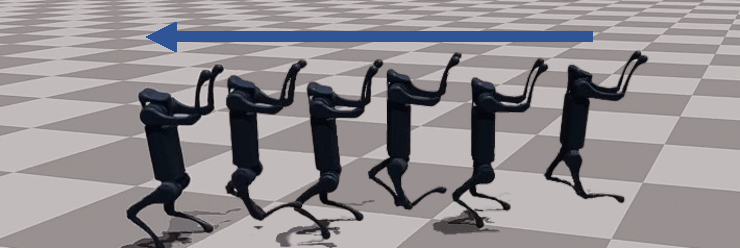
\includegraphics[width=1.0\textwidth]{plane_walk.pdf}
   \caption{Bipedal Walking Posture on Plane Terrain}
   \label{fig:plan_walk}
\end{figure}

Training quadruped robots to walk on four legs is a well-established field in robotics. This course project is based on the famous Rapid Motor Adaptation (RMA) algorithm and its open-source implementation ~\citep{kumar2021rma}. Since the introduction of RMA, other research aimed at enhancing this algorithm has been proposed, including efforts for more precise and safe control ~\citep{SAVIOLO202345}, as well as integration with egocentric vision ~\cite{pmlr-v205-agarwal23a}.

Bipedal robots represent another important research topic, as they often resemble humans and possess significant potential for deployment in real-world industries. Various studies have been proposed for human-like robots with whole-body control ~\citep{cheng2024expressive}. However, these robots often have too many degrees of freedom, making it challenging to define the reward functions necessary for control.


These two topics bring an interesting idea: Can we make the quadruped robots behave like straight-standing dogs, walking bipedally while maintaining balance? Our framework, the RMA algorithm, is known for its rapid adaptation capabilities. However, the teacher training phase also embraces a classic reinforcement learning process with the PPO algorithm ~\citep{schulman2017proximal}, which means we can change the reward functions to make the teacher walk bipedally and then distill the ability to the student. The Unitree A1 quadruped robot possesses only 12 degrees of freedom, fewer than a human-like robot, making this goal more achievable. Recent research ~\citep{li2024learning} has also shown a similar result to let quadruped robots stand bipedally and imitate human action.


Our method includes adjusting the robot's initial rotation and joint angles, modifying the commands, and introducing a set of reward functions designed for bipedal walking on plain and stairs terrains respectively. Our result shows great balancing ability even when climbing steep stairs. The \autoref{fig:plan_walk} shows the bipedal walking posture on the plane terrain with a time interval of 0.1s and the blue arrow represents the moving direction. The \autoref{fig:climb_out} shows the process of climbing out of a square pit with a time interval of 0.5s and the robot keeps a bipedal orientation while climbing the stairs.

\begin{figure}[H]
   \centering
   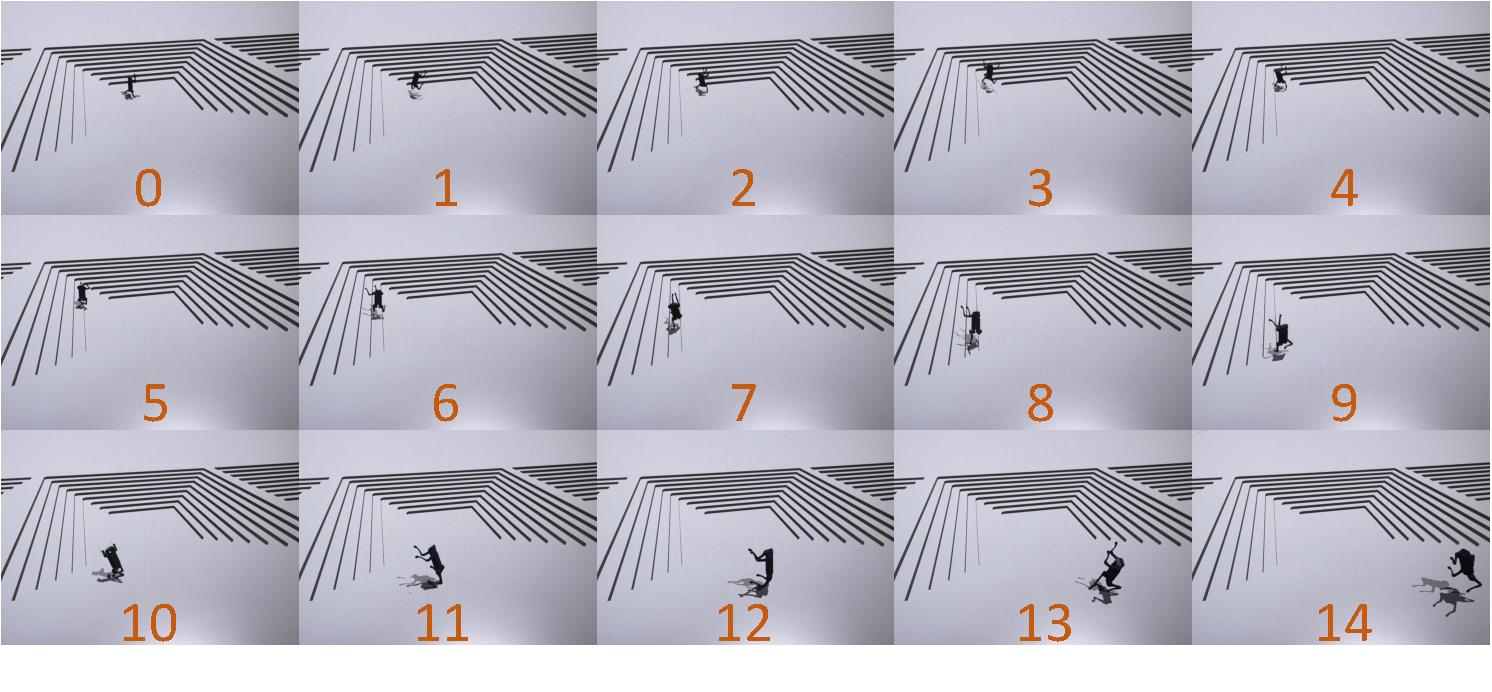
\includegraphics[width=1.0\textwidth]{climb_out.pdf}
   \caption{Process of Climbing out of a Square Pit}
   \label{fig:climb_out}
\end{figure}



\section{Reward-Based Method to Bipedal Walking}

\subsection{Initial Rotation and Joint Angles}

The first challenge is how to make the initially horizontal robot's body (we call it base in the code) stand up since the default body's position and rotation are designed for walking with four legs. When trying to raise the robot's base from the ground to a standing position, it requires an extra training phase to let the network learn how to stand up slowly and robustly. However, when later training from the standing position to walking, the network may be disturbed by the change of rewards and lose the ability to stand up. To solve this problem, we adjust the initial status of the robot, making it ready for bipedal walking at the beginning of the training process. The parameters are shown in \autoref{tab:rotation_parameters} and \autoref{tab:joint_parameters}.

\begin{table}[h]
   \centering
   \begin{tabular}{@{}lcc@{}}
   \toprule
   Dimensions     & Default Parameter (quat) & Bipedal Walking Parameter (quat) \\ \midrule
   \midrule
   x     & 0.0          &  0.0     \\
   y     & 0.0          &  -1.0    \\
   z     & 0.0          &  0.0     \\
   w     & 1.0          &  1.0     \\
   \bottomrule
\end{tabular}
\vspace{-0.5em}
\caption{Rotation Parameters}
\label{tab:rotation_parameters}
\end{table}

\begin{table}[h]
   \centering
   \begin{tabular}{@{}lcc@{}}
   \toprule
   Joint Name       & Default Parameter (rad) & Bipedal Walking Parameter (rad) \\ \midrule
   \midrule
   FL Hip    & 0.1           &  0.2     \\
   RL Hip    & 0.1           &  0.7     \\
   FR Hip    & -0.1          &  0.2     \\
   RR Hip    & -0.1          &  0.7     \\
   FL Thigh  & 0.8           &  -1.0    \\
   RL Thigh  & 1.0           &  1.5     \\
   FR Thigh  & 0.8           &  -1.0    \\
   RR Thigh  & 1.0           &  1.5     \\
   FL Calf   & -1.5          &  -2.2    \\
   RL Calf   & -1.5          &  -0.8    \\
   FR Calf   & -1.5          &  -2.2    \\
   RR Calf   & -1.5          &  -0.8    \\
   \bottomrule
\end{tabular}
\vspace{-0.5em}
\caption{Joint Parameters}
\label{tab:joint_parameters}
\end{table}

\subsection{Commands Modification}

The original training framework assigns an \texttt{x}-axis velocity and a random angular velocity for the \texttt{xy} plane, as shown in ~\autoref{fig:orientation}. When we make the base stand up straight, we must remove all velocity towards the \texttt{x}-axis, as it now represents the vertical direction. The original \texttt{x}-axis velocity is for the \texttt{tracking\_lin\_vel} reward. Therefore, if we want to train the robot to walk bipedally, we should add a \texttt{z}-axis velocity and a reward for \texttt{tracking\_lin\_vel\_z}. Alternatively, we can use another reward, \texttt{lin\_vel\_z}, instead (see \autoref{sec:plane_walking}). This approach avoids modifying too much code in the training framework.

% insert a pdf figure
\begin{figure}[H]
   \centering
   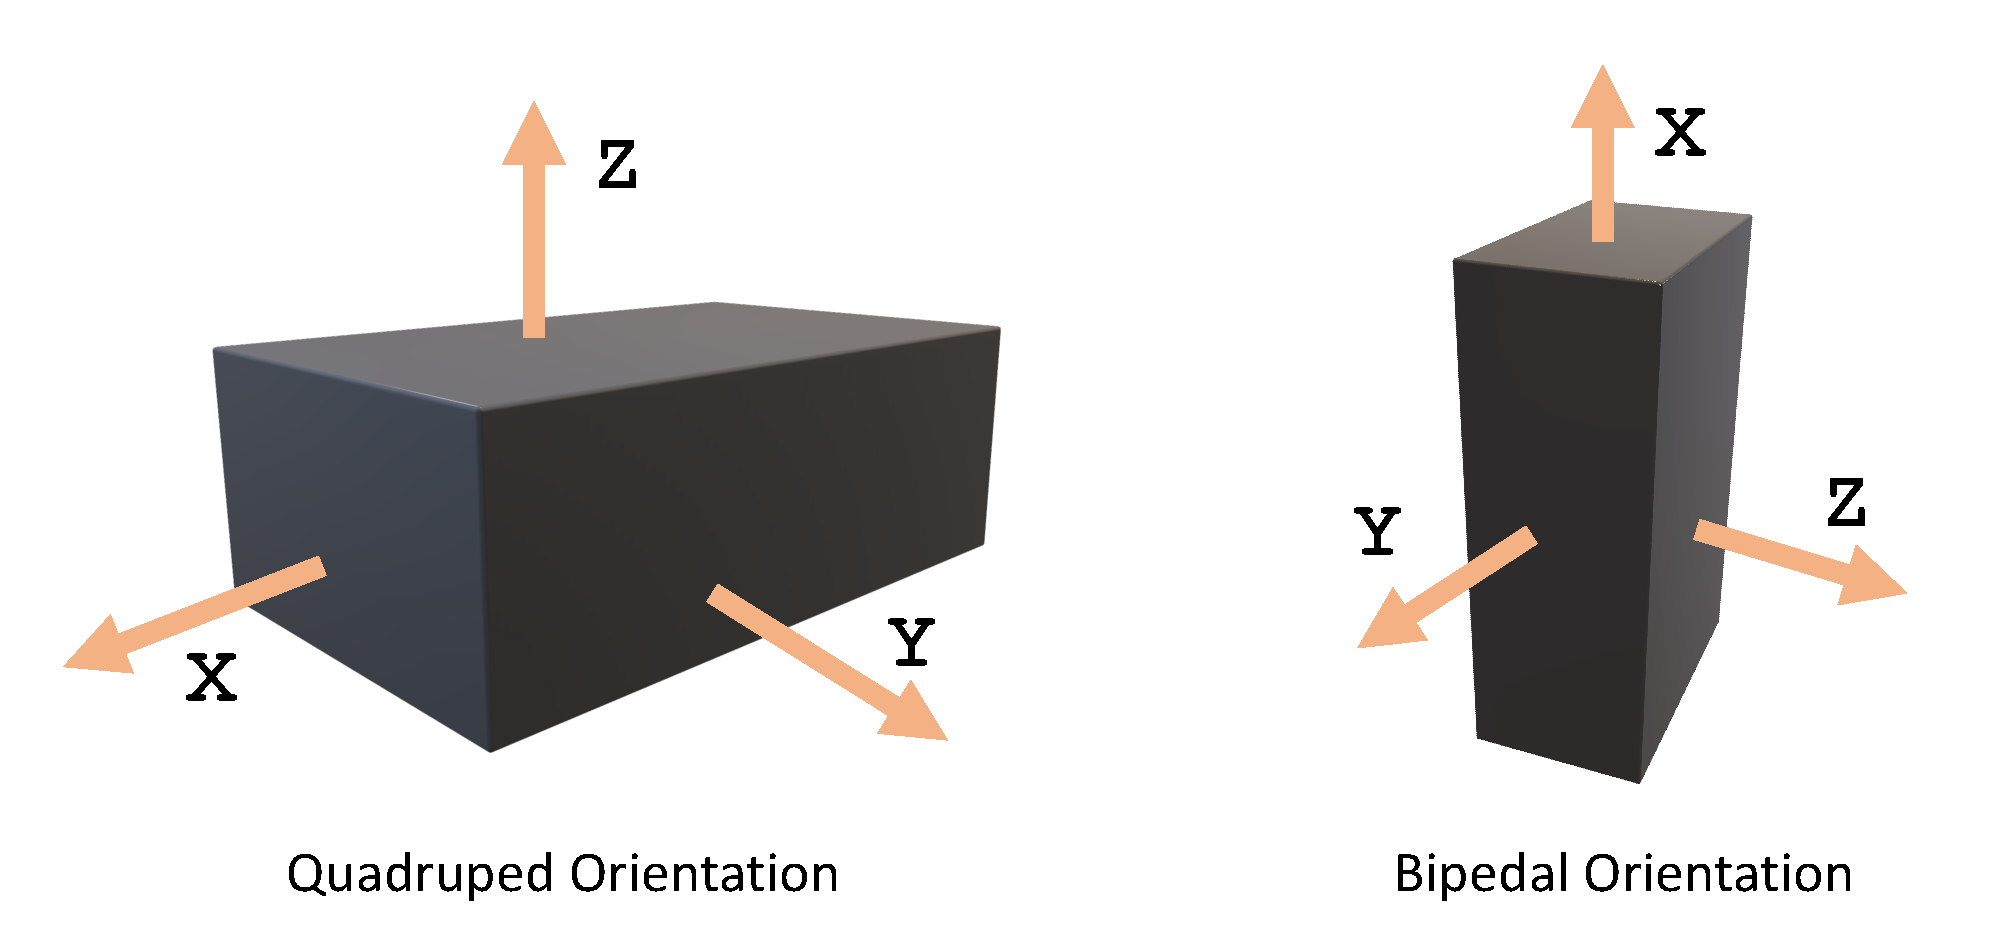
\includegraphics[width=1.0\textwidth]{orientation.pdf}
   \caption{Base Orientation of Quadruped and Bipedal Walking}
   \label{fig:orientation}
\end{figure}


\subsection{Rewards for Plane Walking}
\label{sec:plane_walking}

\subsubsection{Reward Linear Velocity in Z Axis.} 


As demonstrated in the bipedal example of \autoref{fig:orientation}, to encourage forward movement in bipedal walking without directly adding a \texttt{z}-axis velocity to track such direction, it is pivotal to motivate the robot towards forward motion by monitoring the \texttt{z}-axis velocity. To this end, we introduce a reward function, \texttt{reward\_lin\_vel\_z}, as detailed in \autoref{alg:reward_lin_vel_z}. However, during bipedal locomotion, \textit{if the robot falls, the \texttt{z}-axis velocity may surge to excessively high levels, creating the risk of a gradient explosion within the network. To prevent this, we cap the velocity at a maximum value, which is set to 9.0 in our experiments.}

\begin{algorithm}[H]
\caption{Calculate Reward Based on Linear Velocity in Z Axis}
\label{alg:reward_lin_vel_z}
\begin{algorithmic}
\Function{RewardLinVelZ}{}
    \State \textbf{Parameters:} $\text{max\_z\_vel} \gets 9.0$
    \State \textbf{Initialize:} $\text{lin\_vel\_z} \gets \Call{Square}{\text{base\_lin\_vel\_z}}$
    \State \textbf{Return} $\Call{Clip}{\text{lin\_vel\_z}, 0.0, \text{max\_z\_vel}}$
\EndFunction
\end{algorithmic}
\end{algorithm}

\subsubsection{Penalize Other Directions' Linear and Angular Velocity.}

To incentivize forward movement, it's also important to penalize linear and angular velocities in other directions. For instance, a reward function \texttt{penalize\_ang\_vel\_z}, as shown in \autoref{alg:penalize_ang_vel_z}, is added to penalize the angular velocity in the \texttt{z}-axis, corresponding to the robot's rotation around the \texttt{z}-axis. The penalty is calculated using the exponential function of the negative square of the angular velocity, a standard method in reinforcement learning to discourage high values of a variable.

\begin{algorithm}[H]
   \caption{Calculate Panelty Based on Angular Velocity in Z Axis}
   \label{alg:penalize_ang_vel_z}
   \begin{algorithmic}
   \Function{PenalizeAngVelZ}{}
       \State $\text{ang\_vel\_z} \gets \Call{Square}{\text{base\_ang\_vel\_z}}$
       \State \Return $\exp(\text{-ang\_vel\_z} / 0.25)$
   \EndFunction
   \end{algorithmic}
\end{algorithm}

\subsubsection{Reward Bipedal Orientation.}


To promote continuous upright posture in the robot, we introduce a crucial reward function, \texttt{reward\_bipedal\_orientation}, as detailed in \autoref{alg:reward_bipedal_orientation}. This function penalizes the robot's deviation from the vertical axis. The reward is computed as the sum of the squares of the projected gravity vector on the \texttt{yz} plane, which is the plane on which the robot stands. This reward is structured to be positive, with higher values indicating a more vertical orientation of the robot.

\begin{algorithm}[H]
   \caption{Reward Bipedal Orientation}
   \label{alg:reward_bipedal_orientation}
   \begin{algorithmic}
   \Function{RewardBipedalOrientation}{}
       \State \Return $\sum (\Call{Square}{\text{projected\_gravity\_yz}})$ \Comment{Sum over dim=1}
   \EndFunction
   \end{algorithmic}
\end{algorithm}

\subsection{Rewards for Stair Climbing}

The reward functions previously described are optimized for bipedal walking on level ground. \textit{However, applying the same reward structures to stair climbing scenarios within a square pit may result in suboptimal performance, where the robot fails to effectively ascend the stairs. Instead, it may persist in moving in a circular path at the pit's base.} To address this issue, we introduce the \texttt{total\_climb\_height}~\autoref{alg:reward_climb} reward, designed to motivate the robot to tackle the stairs successfully. This reward is computed based on the average of the total climb height, which equals the sum of heights that the robot's root state has ascended, each multiplied by the height interval which denotes the elevation difference between two successive levels of terrain. In our experiments, we set the minimum height threshold at -0.5.

\begin{algorithm}[H]
   \caption{Reward Total Climb Height}
   \label{alg:reward_climb}
   \begin{algorithmic}
   \Function{RewardTotalClimbHeight}{}
       \State $\text{climb\_height} \gets \text{root\_states\_h} + \text{terrain\_levels} \times \text{height\_interval}$
       \State \Return $\Call{Mean}{(\text{climb\_height} - \text{MIN\_H}) \times \text{terrain\_levels}}$
   \EndFunction
   \end{algorithmic}
\end{algorithm}

\section{Experiment Setup}

\subsection{Reward Scales}

The detailed reward functions used in the experiments are as follows:

\begin{itemize}[itemsep=-0.3em]
   \item Torques: Penalize high joint torques.
   \item Action Rate: Penalize high action rate.
   \item \texttt{z} Linear Velocity: Encourage forward movement.
   \item \texttt{x} Linear Velocity: Penalize movement in the \texttt{x} direction.
   \item \texttt{y} Linear Velocity: Penalize movement in the \texttt{y} direction.
   \item \texttt{x} Angular Velocity: Penalize rotation around the \texttt{x} axis.
   \item \texttt{z} Angular Velocity: Penalize rotation around the \texttt{z} axis.
   \item Bipedal Orientation: Encourage vertical orientation.
   \item Bipedal Fall Down: Penalize falling down.
   \item Total Climb Height: Encourage climbing stairs.
   \item Collision: Penalize collision.
\end{itemize}

The reward scales for the plain and stairs terrains are shown in \autoref{tab:reward_scales}.

\begin{table}[H]
   \centering
   \begin{tabular}{@{}lcc@{}}
   \toprule
   Reward Name       & Plain Terrain   & Stairs Terrain \\ \midrule
   torques           &-0.0002          & -0.0002 \\
   action rate       & -0.05           & -0.05 \\
   z linear velocity & 1.0             & 1.5 \\
   x linear velocity & 0.5             & 2.0  \\
   y linear velocity & 1.0             & 1.0  \\
   x angular velocity & 5.0            & 5.0  \\
   z angular velocity & 1.0            & 1.0  \\
   bipedal orientation & -5.0          & -5.0 \\
   bipedal fall down   & -10.0         & -10.0 \\
   total climb height &  0             & 10.0 \\
   collision         & -1.0            & 0 \\
   \bottomrule
   \end{tabular}
\vspace{-0.5em}
\caption{Reward Scales}
\label{tab:reward_scales}
\end{table}


\section{Result and Discussion}

\subsection{Plane Walking}

\begin{figure}[H]
   \centering
   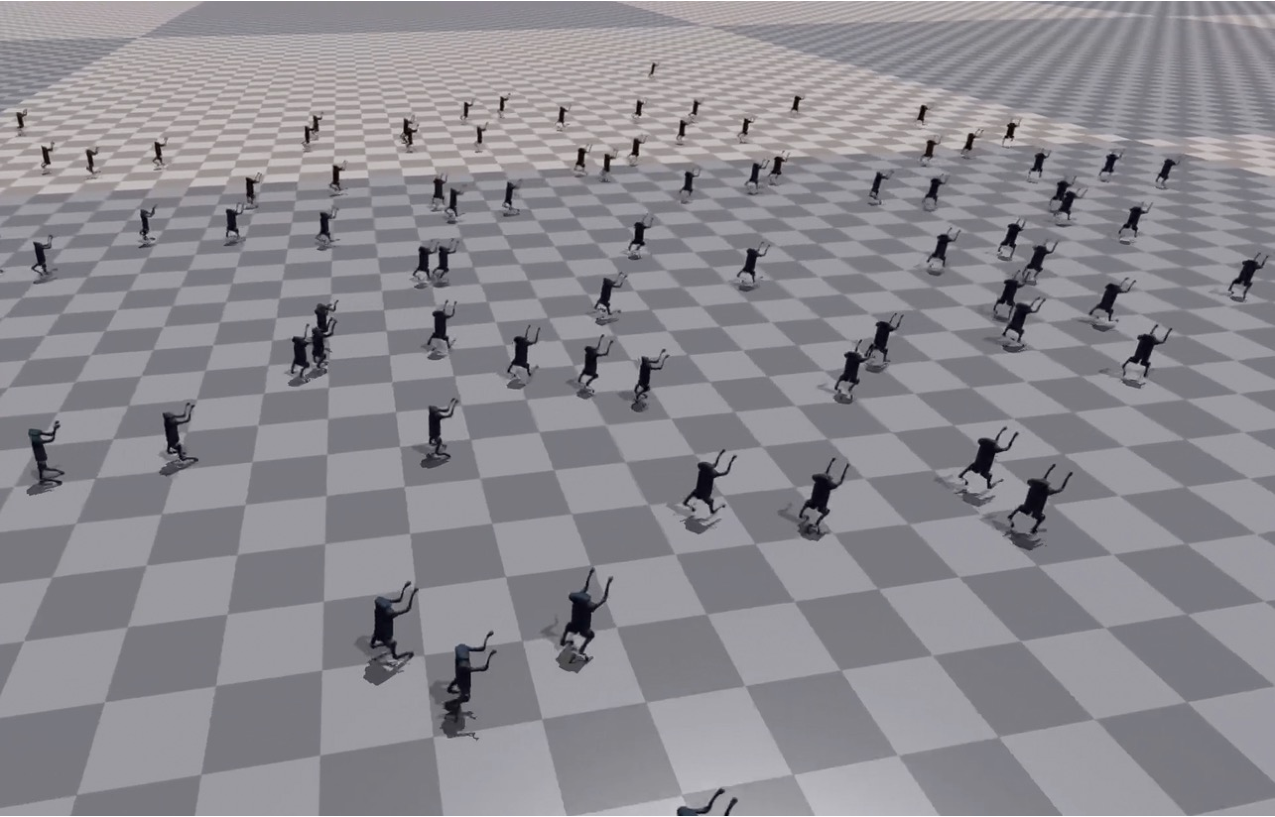
\includegraphics[width=1.0\textwidth]{many_plane_walk.pdf}
   \caption{Bipedal Walking on Plane Terrain}
   \label{fig:many_plane_walk}
\end{figure}

The teacher and student models exhibit comparable performance on flat terrain, as demonstrated in the experiments shown in ~\autoref{fig:many_plane_walk}, where 128 quadruped robots are simulated to walk bipedally across a vast planar surface. Results indicate that the average \texttt{z}-axis velocity can reach up to $3m/s$, with a fall probability within $2\%$.

\subsection{Stairs Climbing}

When it comes to climbing stairs, the teacher model slightly outperforms the student model in terms of balance. With staircases comprising 10 levels of \texttt{trimesh} stairs, each level separated by approximately $0.15$m, the teacher model successfully ascends to the 4th level, whereas the student model peaks at the 3rd level. Across all 10 \texttt{trimesh} stair levels, the teacher model exhibits a lower fall probability, in comparison to the student model's higher fall likelihood of about $10\%$.

\subsection{Stairs Climbing}

\bibliography{rl_paper}
\bibliographystyle{rl_paper}

\appendix
% \section{Appendix}
% You may include other additional sections here.

\end{document}
